% Created by tikzDevice version 0.6.2-92-0ad2792 on 2013-06-06 10:46:52
% !TEX encoding = UTF-8 Unicode
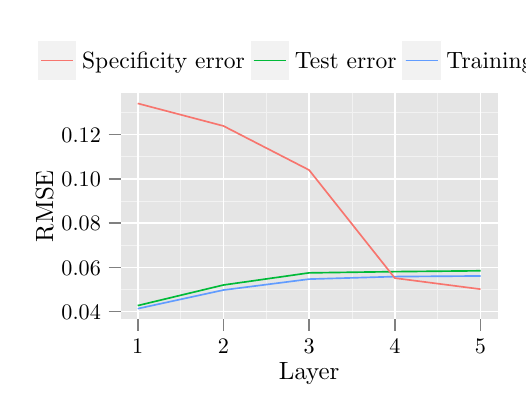
\begin{tikzpicture}[x=1pt,y=1pt]
\tikzstyle{clip}=[]
\definecolor[named]{fillColor}{rgb}{1.00,1.00,1.00}
\path[use as bounding box,fill=fillColor,fill opacity=0.00] (0,0) rectangle (169.83,130.09);
\begin{scope}
\path[clip] ( 33.55, 24.84) rectangle (169.83,106.43);
\definecolor[named]{fillColor}{rgb}{0.90,0.90,0.90}

\path[fill=fillColor] ( 33.55, 24.84) rectangle (169.83,106.43);
\definecolor[named]{drawColor}{rgb}{0.95,0.95,0.95}

\path[draw=drawColor,line width= 0.3pt,line join=round] ( 33.55, 35.47) --
	(169.83, 35.47);

\path[draw=drawColor,line width= 0.3pt,line join=round] ( 33.55, 51.46) --
	(169.83, 51.46);

\path[draw=drawColor,line width= 0.3pt,line join=round] ( 33.55, 67.46) --
	(169.83, 67.46);

\path[draw=drawColor,line width= 0.3pt,line join=round] ( 33.55, 83.45) --
	(169.83, 83.45);

\path[draw=drawColor,line width= 0.3pt,line join=round] ( 33.55, 99.44) --
	(169.83, 99.44);

\path[draw=drawColor,line width= 0.3pt,line join=round] ( 55.23, 24.84) --
	( 55.23,106.43);

\path[draw=drawColor,line width= 0.3pt,line join=round] ( 86.21, 24.84) --
	( 86.21,106.43);

\path[draw=drawColor,line width= 0.3pt,line join=round] (117.18, 24.84) --
	(117.18,106.43);

\path[draw=drawColor,line width= 0.3pt,line join=round] (148.15, 24.84) --
	(148.15,106.43);
\definecolor[named]{drawColor}{rgb}{1.00,1.00,1.00}

\path[draw=drawColor,line width= 0.6pt,line join=round] ( 33.55, 27.47) --
	(169.83, 27.47);

\path[draw=drawColor,line width= 0.6pt,line join=round] ( 33.55, 43.47) --
	(169.83, 43.47);

\path[draw=drawColor,line width= 0.6pt,line join=round] ( 33.55, 59.46) --
	(169.83, 59.46);

\path[draw=drawColor,line width= 0.6pt,line join=round] ( 33.55, 75.45) --
	(169.83, 75.45);

\path[draw=drawColor,line width= 0.6pt,line join=round] ( 33.55, 91.45) --
	(169.83, 91.45);

\path[draw=drawColor,line width= 0.6pt,line join=round] ( 39.75, 24.84) --
	( 39.75,106.43);

\path[draw=drawColor,line width= 0.6pt,line join=round] ( 70.72, 24.84) --
	( 70.72,106.43);

\path[draw=drawColor,line width= 0.6pt,line join=round] (101.69, 24.84) --
	(101.69,106.43);

\path[draw=drawColor,line width= 0.6pt,line join=round] (132.67, 24.84) --
	(132.67,106.43);

\path[draw=drawColor,line width= 0.6pt,line join=round] (163.64, 24.84) --
	(163.64,106.43);
\definecolor[named]{drawColor}{rgb}{0.38,0.61,1.00}

\path[draw=drawColor,line width= 0.6pt,line join=round] ( 39.75, 28.55) --
	( 70.72, 35.28) --
	(101.69, 39.23) --
	(132.67, 40.14) --
	(163.64, 40.37);
\definecolor[named]{drawColor}{rgb}{0.00,0.73,0.22}

\path[draw=drawColor,line width= 0.6pt,line join=round] ( 39.75, 29.66) --
	( 70.72, 37.10) --
	(101.69, 41.49) --
	(132.67, 41.93) --
	(163.64, 42.24);
\definecolor[named]{drawColor}{rgb}{0.97,0.46,0.43}

\path[draw=drawColor,line width= 0.6pt,line join=round] ( 39.75,102.72) --
	( 70.72, 94.58) --
	(101.69, 78.65) --
	(132.67, 39.60) --
	(163.64, 35.60);
\end{scope}
\begin{scope}
\path[clip] (  0.00,  0.00) rectangle (169.83,130.09);
\definecolor[named]{drawColor}{rgb}{0.00,0.00,0.00}

\node[text=drawColor,anchor=base east,inner sep=0pt, outer sep=0pt, scale=  0.80] at ( 26.44, 24.72) {0.04};

\node[text=drawColor,anchor=base east,inner sep=0pt, outer sep=0pt, scale=  0.80] at ( 26.44, 40.71) {0.06};

\node[text=drawColor,anchor=base east,inner sep=0pt, outer sep=0pt, scale=  0.80] at ( 26.44, 56.71) {0.08};

\node[text=drawColor,anchor=base east,inner sep=0pt, outer sep=0pt, scale=  0.80] at ( 26.44, 72.70) {0.10};

\node[text=drawColor,anchor=base east,inner sep=0pt, outer sep=0pt, scale=  0.80] at ( 26.44, 88.69) {0.12};
\end{scope}
\begin{scope}
\path[clip] (  0.00,  0.00) rectangle (169.83,130.09);
\definecolor[named]{drawColor}{rgb}{0.50,0.50,0.50}

\path[draw=drawColor,line width= 0.6pt,line join=round] ( 29.29, 27.47) --
	( 33.55, 27.47);

\path[draw=drawColor,line width= 0.6pt,line join=round] ( 29.29, 43.47) --
	( 33.55, 43.47);

\path[draw=drawColor,line width= 0.6pt,line join=round] ( 29.29, 59.46) --
	( 33.55, 59.46);

\path[draw=drawColor,line width= 0.6pt,line join=round] ( 29.29, 75.45) --
	( 33.55, 75.45);

\path[draw=drawColor,line width= 0.6pt,line join=round] ( 29.29, 91.45) --
	( 33.55, 91.45);
\end{scope}
\begin{scope}
\path[clip] (  0.00,  0.00) rectangle (169.83,130.09);
\definecolor[named]{drawColor}{rgb}{0.50,0.50,0.50}

\path[draw=drawColor,line width= 0.6pt,line join=round] ( 39.75, 20.58) --
	( 39.75, 24.84);

\path[draw=drawColor,line width= 0.6pt,line join=round] ( 70.72, 20.58) --
	( 70.72, 24.84);

\path[draw=drawColor,line width= 0.6pt,line join=round] (101.69, 20.58) --
	(101.69, 24.84);

\path[draw=drawColor,line width= 0.6pt,line join=round] (132.67, 20.58) --
	(132.67, 24.84);

\path[draw=drawColor,line width= 0.6pt,line join=round] (163.64, 20.58) --
	(163.64, 24.84);
\end{scope}
\begin{scope}
\path[clip] (  0.00,  0.00) rectangle (169.83,130.09);
\definecolor[named]{drawColor}{rgb}{0.00,0.00,0.00}

\node[text=drawColor,anchor=base,inner sep=0pt, outer sep=0pt, scale=  0.80] at ( 39.75, 12.22) {1};

\node[text=drawColor,anchor=base,inner sep=0pt, outer sep=0pt, scale=  0.80] at ( 70.72, 12.22) {2};

\node[text=drawColor,anchor=base,inner sep=0pt, outer sep=0pt, scale=  0.80] at (101.69, 12.22) {3};

\node[text=drawColor,anchor=base,inner sep=0pt, outer sep=0pt, scale=  0.80] at (132.67, 12.22) {4};

\node[text=drawColor,anchor=base,inner sep=0pt, outer sep=0pt, scale=  0.80] at (163.64, 12.22) {5};
\end{scope}
\begin{scope}
\path[clip] (  0.00,  0.00) rectangle (169.83,130.09);
\definecolor[named]{drawColor}{rgb}{0.00,0.00,0.00}

\node[text=drawColor,anchor=base,inner sep=0pt, outer sep=0pt, scale=  0.90] at (101.69,  3.01) {Layer};
\end{scope}
\begin{scope}
\path[clip] (  0.00,  0.00) rectangle (169.83,130.09);
\definecolor[named]{drawColor}{rgb}{0.00,0.00,0.00}

\node[text=drawColor,rotate= 90.00,anchor=base,inner sep=0pt, outer sep=0pt, scale=  0.90] at (  9.21, 65.64) {RMSE};
\end{scope}
\begin{scope}
\path[clip] (  0.00,  0.00) rectangle (169.83,130.09);
\definecolor[named]{fillColor}{rgb}{1.00,1.00,1.00}

\path[fill=fillColor] ( -4.49,106.76) rectangle (207.88,129.75);
\end{scope}
\begin{scope}
\path[clip] (  0.00,  0.00) rectangle (169.83,130.09);
\definecolor[named]{drawColor}{rgb}{1.00,1.00,1.00}
\definecolor[named]{fillColor}{rgb}{0.95,0.95,0.95}

\path[draw=drawColor,line width= 0.6pt,line join=round,line cap=round,fill=fillColor] (  3.39,111.03) rectangle ( 17.85,125.49);
\end{scope}
\begin{scope}
\path[clip] (  0.00,  0.00) rectangle (169.83,130.09);
\definecolor[named]{drawColor}{rgb}{0.97,0.46,0.43}

\path[draw=drawColor,line width= 0.6pt,line join=round] (  4.84,118.26) -- ( 16.40,118.26);
\end{scope}
\begin{scope}
\path[clip] (  0.00,  0.00) rectangle (169.83,130.09);
\definecolor[named]{drawColor}{rgb}{0.97,0.46,0.43}

\path[draw=drawColor,line width= 0.6pt,line join=round] (  4.84,118.26) -- ( 16.40,118.26);
\end{scope}
\begin{scope}
\path[clip] (  0.00,  0.00) rectangle (169.83,130.09);
\definecolor[named]{drawColor}{rgb}{0.97,0.46,0.43}

\path[draw=drawColor,line width= 0.6pt,line join=round] (  4.84,118.26) -- ( 16.40,118.26);
\end{scope}
\begin{scope}
\path[clip] (  0.00,  0.00) rectangle (169.83,130.09);
\definecolor[named]{drawColor}{rgb}{1.00,1.00,1.00}
\definecolor[named]{fillColor}{rgb}{0.95,0.95,0.95}

\path[draw=drawColor,line width= 0.6pt,line join=round,line cap=round,fill=fillColor] ( 80.31,111.03) rectangle ( 94.76,125.49);
\end{scope}
\begin{scope}
\path[clip] (  0.00,  0.00) rectangle (169.83,130.09);
\definecolor[named]{drawColor}{rgb}{0.00,0.73,0.22}

\path[draw=drawColor,line width= 0.6pt,line join=round] ( 81.76,118.26) -- ( 93.32,118.26);
\end{scope}
\begin{scope}
\path[clip] (  0.00,  0.00) rectangle (169.83,130.09);
\definecolor[named]{drawColor}{rgb}{0.00,0.73,0.22}

\path[draw=drawColor,line width= 0.6pt,line join=round] ( 81.76,118.26) -- ( 93.32,118.26);
\end{scope}
\begin{scope}
\path[clip] (  0.00,  0.00) rectangle (169.83,130.09);
\definecolor[named]{drawColor}{rgb}{0.00,0.73,0.22}

\path[draw=drawColor,line width= 0.6pt,line join=round] ( 81.76,118.26) -- ( 93.32,118.26);
\end{scope}
\begin{scope}
\path[clip] (  0.00,  0.00) rectangle (169.83,130.09);
\definecolor[named]{drawColor}{rgb}{1.00,1.00,1.00}
\definecolor[named]{fillColor}{rgb}{0.95,0.95,0.95}

\path[draw=drawColor,line width= 0.6pt,line join=round,line cap=round,fill=fillColor] (135.08,111.03) rectangle (149.54,125.49);
\end{scope}
\begin{scope}
\path[clip] (  0.00,  0.00) rectangle (169.83,130.09);
\definecolor[named]{drawColor}{rgb}{0.38,0.61,1.00}

\path[draw=drawColor,line width= 0.6pt,line join=round] (136.53,118.26) -- (148.09,118.26);
\end{scope}
\begin{scope}
\path[clip] (  0.00,  0.00) rectangle (169.83,130.09);
\definecolor[named]{drawColor}{rgb}{0.38,0.61,1.00}

\path[draw=drawColor,line width= 0.6pt,line join=round] (136.53,118.26) -- (148.09,118.26);
\end{scope}
\begin{scope}
\path[clip] (  0.00,  0.00) rectangle (169.83,130.09);
\definecolor[named]{drawColor}{rgb}{0.38,0.61,1.00}

\path[draw=drawColor,line width= 0.6pt,line join=round] (136.53,118.26) -- (148.09,118.26);
\end{scope}
\begin{scope}
\path[clip] (  0.00,  0.00) rectangle (169.83,130.09);
\definecolor[named]{drawColor}{rgb}{0.00,0.00,0.00}

\node[text=drawColor,anchor=base west,inner sep=0pt, outer sep=0pt, scale=  0.85] at ( 19.65,115.33) {Specificity error};
\end{scope}
\begin{scope}
\path[clip] (  0.00,  0.00) rectangle (169.83,130.09);
\definecolor[named]{drawColor}{rgb}{0.00,0.00,0.00}

\node[text=drawColor,anchor=base west,inner sep=0pt, outer sep=0pt, scale=  0.85] at ( 96.57,115.33) {Test error};
\end{scope}
\begin{scope}
\path[clip] (  0.00,  0.00) rectangle (169.83,130.09);
\definecolor[named]{drawColor}{rgb}{0.00,0.00,0.00}

\node[text=drawColor,anchor=base west,inner sep=0pt, outer sep=0pt, scale=  0.85] at (151.34,115.33) {Training error};
\end{scope}
\end{tikzpicture}
